
Today radio resources become expensive due to the huge number of used systems. Smart ways to radio resource allocation is getting more and more important in wireless communication. The spectrum sharing ways should be done very carefully, to hold interference for legal systems. Additional approaches to increase frequency efficiency raise the complexity of the wireless systems \cite{Book32}. 
The fourth generation was the OFDM system. The OFDM system doesn't provide the necessary inter-system interference level for the nearby frequency bands \cite{Book34}\cite{Book35}. In addition, the OFDM system based on the orthogonality between different sub-carriers.  OFDM use additional time domain filter to archive orthogonality between sub-carriers.  In the next generation proposed more efficient frequency resources usage. A new technique  is called generalized frequency division modulation. It based on the non-orthogonal sub-carrier location \cite{Book34} \cite{Book33}. The transmitter put the sub-carrier frequencies with overlap. The system provides such behaviour with root-raised cosine filters instead of the $sinc$ filters. Selected approach allow decreasing out-of-band radiation, but introducing self-interference in the system. The self-interference decrease performance in the system.  New filter design add flexibility to the system because has the adjusting coefficient. The system adjust self-interference to find the trade-off between performance and frequency efficiency. Another requirement is spectrum-sensing approach for the transmitter and receiver side. For that case receiver should estimate both the transmitted symbols and the used sub-carriers. This task has uncertainty in case if all symbols is unknown. To estimate both of the variables the receiver should know additional information. The receiver may know the first column of the transmitted symbol matrix. All explained approaches make receiver and transmitter more complex. The receiver in the new system must solve much more complicated task to provide the same BER. The algorithms to symbol estimation also become more complicated.   There is a way to simplify the definition of the modulation matrix. We can use the tensor algebra and explain the transmission with a more natural and easy way. 
\section{Tensor based processing}\label{sec:TBP}
A tensor is a multidimensional array \eqref{i_1}\cite{Book6}. In other words, the Nth-order tensor is a matrix which has elements over N different dimensions. The first and second order tensors correspond to the arrays and matrices from linear algebra\cite{Book12}. The tensors, which has number of dimension higher or equal to three are called higher order tensors. 
\begin{align}
\mathcal{X} \in \compl^{I_1\times I_2\cdots I_N}
\label{i_1}
\end{align}
The order of the tensor is the number of dimensions which tensor has. In this thesis scalars are denoted by the lowercase letters e.g. a. The arrays are denoted by boldface lowercase letters e.g. $\mathbf{a}$. The matrices are written as the boldface capital letters e.g. $\mathbf{A}$. Higher order tensors are denoted by capital calligraphic letters e.g. $\mathcal{A}$.
Tensors explain data with high number of variables in a more natural way. Tensor based explanation of the data allow to consider all dependencies between dimensions of the data. 
The N-th order unfolding of the tensor is the stacked version of the tensor with respect to the N-th dimension \eqref{i_2}\eqref{i_3}\eqref{i_4}\eqref{i_5}\cite{Book16}. In the N-th order unfolding the elements of the each columns is fixed for the all dimensions except N. The N-th order unfolding has the number of row equal to the N dimension size, the number of the column equal to the product between other dimensions. The order of the columns are defines as the notation of the unfolding. In this paper is considered MATLAB ordering\cite{Book19}. The MATLAB notation change dimensions in the increasing order.
\begin{align}
\mathcal{X}_{:,:,1}=\begin{bmatrix}
1&3\\ 
0&1\\
\end{bmatrix} \; \mathcal{X}_{:,:,2}=\begin{bmatrix}
2&-3\\ 
-1&2\\
\end{bmatrix}
\label{i_2}
\end{align}
\begin{align}
\mathcal{X}_{[1]}=\begin{bmatrix}
1&3&2&-3\\ 
0&1&-1&2\\
\end{bmatrix}
\label{i_3}
\end{align}
\begin{align}
\mathcal{X}_{[2]}=\begin{bmatrix}
1&0&2&-1\\ 
3&1&-3&2\\
\end{bmatrix}
\label{i_4}
\end{align}
\begin{align}
\mathcal{X}_{[3]}=\begin{bmatrix}
1&0&3&1\\ 
2&-1&-3&2\\
\end{bmatrix}
\label{i_5}
\end{align}
The N-th order tensor is rank-one if it can be presented as the outer products of N vectors.
The Hitchcock proposes the tensor decomposition  in the 1927. He expressed the higher order tensor as the sum of the rank-one tensors \eqref{i_6}\eqref{i_7}.
\begin{align}
\mathcal{X}=\sum_{r=1}^R \mathbf{a}_r \circ \mathbf{b}_r \circ \mathbf{c}_r
\label{i_6}
\end{align}
\begin{align}
\mathcal{X}\in \compl^{I_1\times I_2\times I_3} \mathbf{a}_r\in \compl^{I_1\times 1} \mathbf{b}_r\in \compl^{I_2\times 1} \mathbf{c}_r\in \compl^{I_3\times 1}
\label{i_7}
\end{align}
The  tensor can be decomposed as the number of rank-one tensors. Decomposition called "CP" or CANDECOMP/PARAFAC decomposition\cite{Book6}. The "CP" decomposition factorizes the tensor into a sum of rank-one tensors components. Sum of rank-one tensor can be presented in another form \eqref{i_8} . The arrays corresponding to the same dimension can be stacked in the one matrix for each dimension respectively. This notation is called the "factor matrices". The factor matrices present the tensor unfolding in simplified form \eqref{i_10}\eqref{i_11}\eqref{i_12}.
\begin{align}
\mathcal{X}=\mathcal{I}\times_1 \mathbf{A} \times_2\mathbf{B} \times_3 \mathbf{C}
\label{i_8}
\end{align}
\begin{align}
\mathcal{X}\times_n \mathbf{A}=\mathbf{A}\mathcal{X}_{[n]}
\end{align}
\begin{align}
\mathbf{A}=\begin{bmatrix}
\mathbf{a}_1&\mathbf{a}_2\cdots \mathbf{a}_R\\
\end{bmatrix}
\label{i_9}
\end{align}
\begin{align}
\mathcal{X}_{[1]}=\mathbf{A}(\mathbf{C}\diamond \mathbf{B})^T
\label{i_10}
\end{align}
\begin{align}
\mathcal{X}_{[2]}=\mathbf{B}(\mathbf{C}\diamond \mathbf{A})^T
\label{i_11}
\end{align}
\begin{align}
\mathcal{X}_{[3]}=\mathbf{C}(\mathbf{A}\diamond \mathbf{B})^T
\label{i_12}
\end{align}
There are many decomposition algorithms. One of the most popular is the Alternating least squares algorithm. The algorithm is explained as follows:
\begin{itemize}
\item Set $\mathbf{C}$ and $\mathbf{B}$ as random valued matrices
\item Solve equation for the first unfolding with respect to the $\mathbf{A}$ with given $\mathbf{C}$ and $\mathbf{B}$
\item Solve equation for the first unfolding with respect to the $\mathbf{B}$ with given $\mathbf{C}$ and $\mathbf{A}$
\item Solve equation for the first unfolding with respect to the $\mathbf{C}$ with given $\mathbf{A}$ and $\mathbf{B}$
\item Check the tolerance of residual, if residual higher than tolerance repeat from step 2
\end{itemize}
\subsection{PARATUCK2 model}\label{part:PTM}
The PARATUCK2 model is the combination between the PARAFAC \cite{Book12} and TUCKER2 \cite{Book6} tensor models. The PARATUCK2 \cite{Book6} combines decomposition between five different matrices into one tensor. The
PARATUCK2 model in general is explained as the three-dimensional
tensor and is defined in scalar form as given in \eqref{p_1} \cite{Book26}
\begin{align}
x_{i_1,i_2,t}=\sum^{F}_{f=1} \sum^{T_s}_{t_s=1}a_{i_1,f}c^{[a]}_{t,f}s_{f,t_s}c^{[b]}_{f,t_s}b_{i_2,t_s}
\label{p_1}
\end{align}
\begin{align*}
\mathcal{X} \in \compl^{I_1 \times, I_2 \times T} \mathbf{A} \in \compl^{I_1 \times F} \mathbf{B} \in \compl^{I_2 \times T_s}
\end{align*}
\begin{align*}
\mathbf{C}^{[a]} \in \compl^{T \times F} \mathbf{C}^{[b]} \in \compl^{T \times T_s}
\end{align*}
where $x_{i_1,i_2,t}$ is $(i_1,i_2,t)$ -th entry of the resulting tensor $\mathcal{X} \in \compl^{I_1 \times I_2 \times T }$.The $\mathbf{S}$ matrix is the core matrix of the PARATUCK2 model. The matrices $\mathbf{A}$ and $\mathbf{B}$ show connection
between the core matrix $\mathbf{S}$ to the first and the second dimensions. The $\mathbf{C^{[a]}}$ and $\mathbf{C^{[b]}}$ are the scaling matrices defining the $\mathbf{A}$ and $\mathbf{B}$ relations to the core matrix $\mathbf{S}$.  Every element of the core matrix links the $\mathbf{A}$ and $\mathbf{B}$ matrices as the scaling coefficient\cite{Book12}.

The PARATUCK2 model possible to write in the two forms: slice-by-slice multiplication form and vectorized form.
In the  slice-by-slice product form the equation for the tensor is written for each slice separately \eqref{p_2}. Explained form allow writing the model as matrix multiplication with change only in two matrices for different slices.  The $\mathbf{C^{[a]}}$ and $\mathbf{C^{[b]}}$ is written as the tensor with elements on the diagonal in the first and second dimension. The linear combination between tensors become the scaling coefficients for columns in the each $i_3$ point. In that case the PARATUCK2 model will be written as the slice-wise multiplication \eqref{p_2} over the matrices $\mathbf{A} $ and $\mathbf{B} $ from the corresponding side with diagonalized tensors $\mathbf{C^{[a]}}$ and $\mathbf{C^{[b]}}$ for the corresponding slice\cite{Book12}.
\begin{align}
\mathbf{X}_{:,:,i}=\mathbf{A}\cdot diag(\mathbf{C^{[a]}}_{:,i})\cdot \mathbf{S}\cdot diag(\mathbf{C^{[b]}}_{:,i})\cdot \mathbf{B}
\label{p_2}
\end{align}
Vectorized form of tensor $\mathcal{X}$ is another form to write the PARATUCK2 model\eqref{p_3} . We can write three equations with respect to the vectorized versions of the $\mathbf{A}$ \eqref{p_4},$\mathbf{S}$\eqref{p_3},$\mathbf{B}$\eqref{p_5}\cite{Book26}.Structure of the tensor in the defined equation is lost,  because we have only vectorized version of the tensor. The slice-wise model is replaced via matrix operations and allow operating with matrices instead of the tensors of different matrix operation for different slices\cite{Book26}.
\begin{align}
vec(\mathcal{X})=\begin{bmatrix}
(\mathbf{C^{[a]T}} \diamond \mathbf{C^{[b]T}})^T \diamond (vec(\mathbf{A}_{1,:})\otimes \mathbf{B})\\
(\mathbf{C^{[a]T}} \diamond \mathbf{C^{[b]T}})^T \diamond (vec(\mathbf{A}_{2,:})\otimes \mathbf{B})\\
\vdots \\
(\mathbf{C^{[a]T}} \diamond \mathbf{C^{[b]T}})^T \diamond (vec(\mathbf{A}_{I_1,:})\otimes \mathbf{B})\\
\end{bmatrix} vec(\mathbf{S})
\label{p_3}
\end{align}
\begin{align}
vec(\mathcal{X})=(\mathbf{I} \otimes(((\mathbf{B}\diamond \mathbf{C}^{[b]}) \cdot \mathbf{S}^T) \odot \mathbf{C}^{[a]}) )vec(\mathbf{A})
\label{p_4}
\end{align}
\begin{align}
vec(\mathcal{X})=(\mathbf{I} \otimes (((\mathbf{A}\diamond \mathbf{C}^{[a]}) \cdot \mathbf{S}) \odot \mathbf{C}^{[b]} ))vec(\mathbf{B})
\label{p_5}
\end{align}
 The PARATUCK2 model in vectorized form possible to simplify with the Hadamard and the Khatri-Rao product notation in case if $\mathbf{A}$ and $\mathbf{B}$ have only one dimension \eqref{i_2}. The definition is provided via vectorization over the resulting tensor.The PARATUCK2 model become array in the third dimension.    The PARATUCK2 with one dimensioned $\mathbf{a}$ and $\mathbf{b}$  model is explained in the matrix notation with two different equation  \eqref{p_6}\cite{Book26}. The difference between equations is order of the multiplication between matrices. The Khatri-Rao and the Hadamard product is sensible to the multiplication order and change of the multiplication order, change overall model construction. A transpose of the $\mathbf{X}$ also change the matrix multiplication order.
\begin{align}
vec(\mathcal{X})^T=\mathbf{a}\cdot (\mathbf{C}^{[a]T} \odot (\mathbf{S}\cdot (\mathbf{C}^{[b]}\diamond \mathbf{b}^T)^T))
\label{p_6}
\end{align}
%\begin{align}
%vec(\mathcal{X})^T=\mathbf{b}^T\cdot (\mathbf{C}^{[b]T} \odot (\mathbf{S}^T  \cdot (\mathbf{C}^{[a]}\diamond \mathbf{a})^T))
%\label{p_7}
%\end{align}
%\begin{align}
%vec(\mathcal{X})=(((\mathbf{a}\diamond \mathbf{C}^{[a]}) \cdot \mathbf{S}) \odot \mathbf{C}^{[b]} )\mathbf{b})
%\label{p_8}
%\end{align}
%\begin{align}
%vec(\mathcal{X})=(((\mathbf{b}^T\diamond \mathbf{C}^{[b]}) \cdot \mathbf{S}^T) \odot \mathbf{C}^{[a]}) \mathbf{a}^T) 
%\label{p_9}
%\end{align}
%\begin{align*}
%\mathcal{X} \in \compl^{1 \times 1 \times T} 
%\mathbf{a} \in \compl^{1 \times F} 
%\mathbf{b} \in \compl^{T_s \times 1}
%\end{align*}
\begin{align*}
\mathbf{C}^{[a]} \in \compl^{T \times F}
\mathbf{C}^{[b]} \in \compl^{T \times T_s}
\mathbf{S} \in \compl^{F \times T_s}
\end{align*}
 
The explained PARATUCK2 model will be used in the further work to define the GFDM system and allow to calculate solutions in the more natural form.
\section{Generalized frequency division multiplexing systems}\label{sec:GFDM}
The generalized frequency division modulation (GFDM) is the new approach to increase the spectral efficiency of the data transmission systems\cite{Book25} \cite{Book22}. The GFDM is extended version of the orthogonal frequency division modulation system with the additional overlapping in the frequency domain. The main principle of the GFDM system is transmission of the symbols during one transmission block on the number of sub-carriers and in the number of the time slots. Each symbol corresponding to the certain time slot is modulated with time domain filter. Time domain filter provides certain envelope in the time domain. The GFDM system use special form of the time domain filters which has the overlap with the symbols on the nearest sub-carriers. This approach provide more dense symbol arrangement in the frequency domain\cite{Book24}.
\subsection{Time filter construction principles}\label{part:TFCP}
 In the GFDM system are used two main filters: raised cosine and root-raised cosine filter instead of the $sinc$ pulse-shaping filter in the OFDM system.  Both of the filters have the variable coefficient $\alpha$ which allow to adjust the overlapping in the frequency domain from $0$ to $1$ where when $\alpha=0$ the overlap is minimal and  when $\alpha=1$ the overlap is maximal\cite{Book30}\cite{Book21}. That variable increase significantly inter-symbol interference and inter-channel interference and allow pitting symbols more dense than in the OFDM system. The additional price for efficient frequency usage is receiver complexity. The receiver must separate all time symbols inside the one transmission block, even if the symbols is overlapped. 
 
 The raised cosine filter envelope is provided in the \eqref{g_1} below from the \cite{Book5} paper. In the \eqref{g_1} $T$ is the symbol duration in the time samples, and $\alpha$ is $roll-off$ factor, which is described above\cite{Book33}. The envelope of the raised cosine filter with different $roll-off$ factors is presented in the \ref{fg_1}. The following frequency envelope is presented in the \ref{fg_2}.
\begin{align}
\begin{matrix}
h(t)&=&\left\{
\begin{matrix}
\frac{\pi sinc(\frac{1}{2\alpha})}{4}& t=\pm \frac{T}{2\alpha}\\
sinc(1/T)\frac{cos(\pi \alpha t/T)}{1-(2 \alpha t /T)^2}&otherwise\\
\end{matrix} \right.
\end{matrix}
\label{g_1}
\end{align}
\begin{figure}[H]
\centering
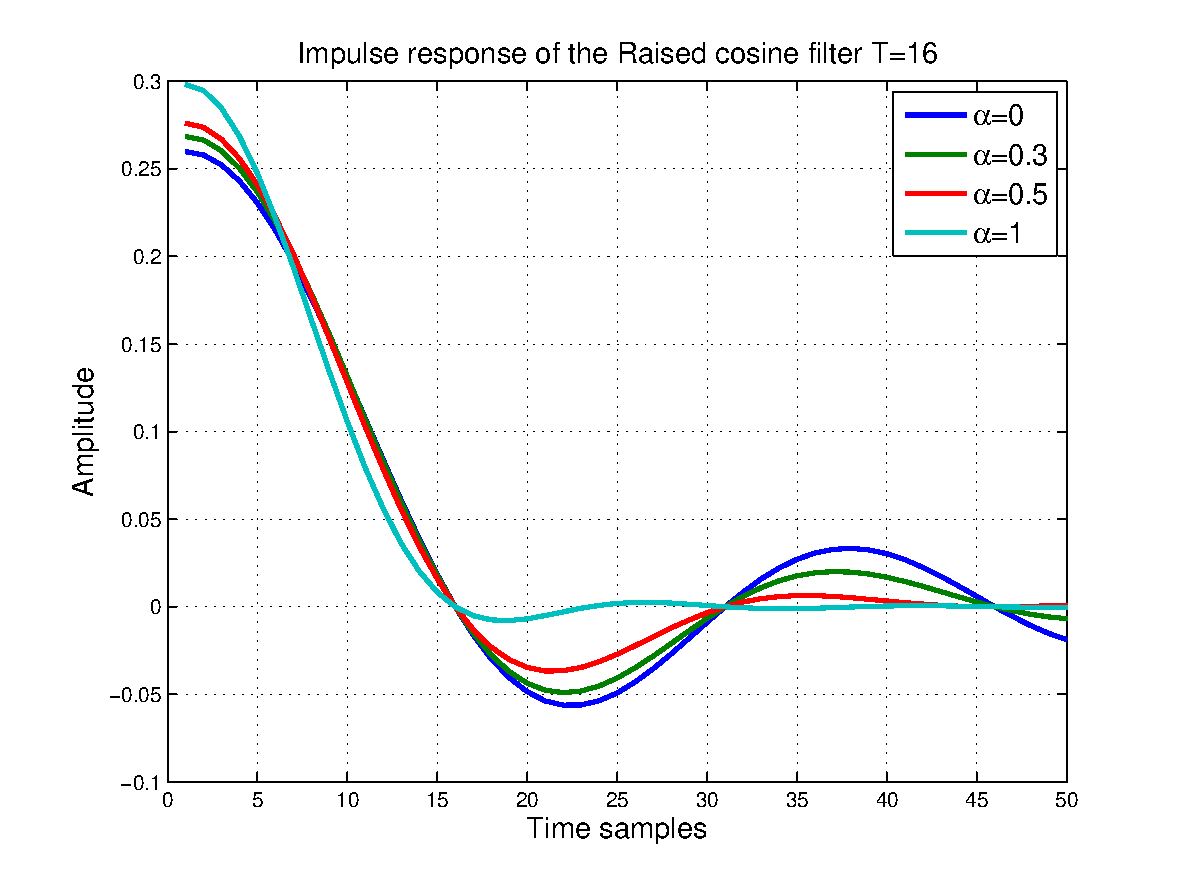
\includegraphics[width=0.9\columnwidth]{RC_time.eps}
\caption{\textit{Impulse response of the raised cosine filter with different roll-off factor $\alpha$}}
\label{fg_1}
\end{figure}
\begin{figure}[H]
\centering
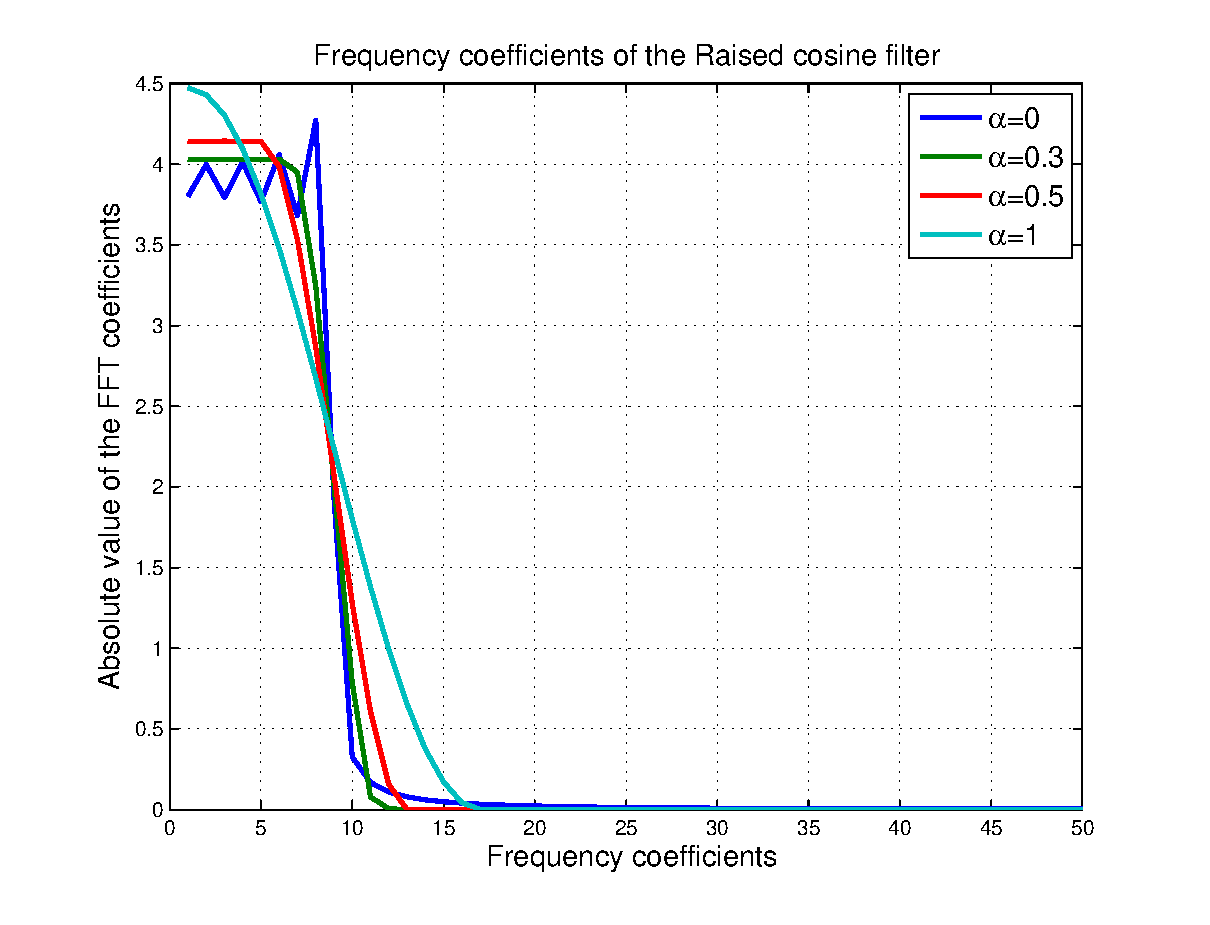
\includegraphics[width=0.9\columnwidth]{RC_freq.eps}
\caption{\textit{Frequency envelope of the raised cosine filter with different roll-off factor $\alpha$}} 
\label{fg_2}
\end{figure}
The root-raised cosine filter equation is provided in the \eqref{g_2} and given in the \cite{Book34} paper. In the \eqref{g_2} $T$ is the symbol duration in the time samples, and $\alpha$ is $roll-off$ factor, which was described above.The envelope of the root-raised cosine filter with different $roll-off$ factors is presented in the \ref{fg_3}. The following frequency envelope is presented in the \ref{fg_4}.
\begin{figure}[H]
\centering
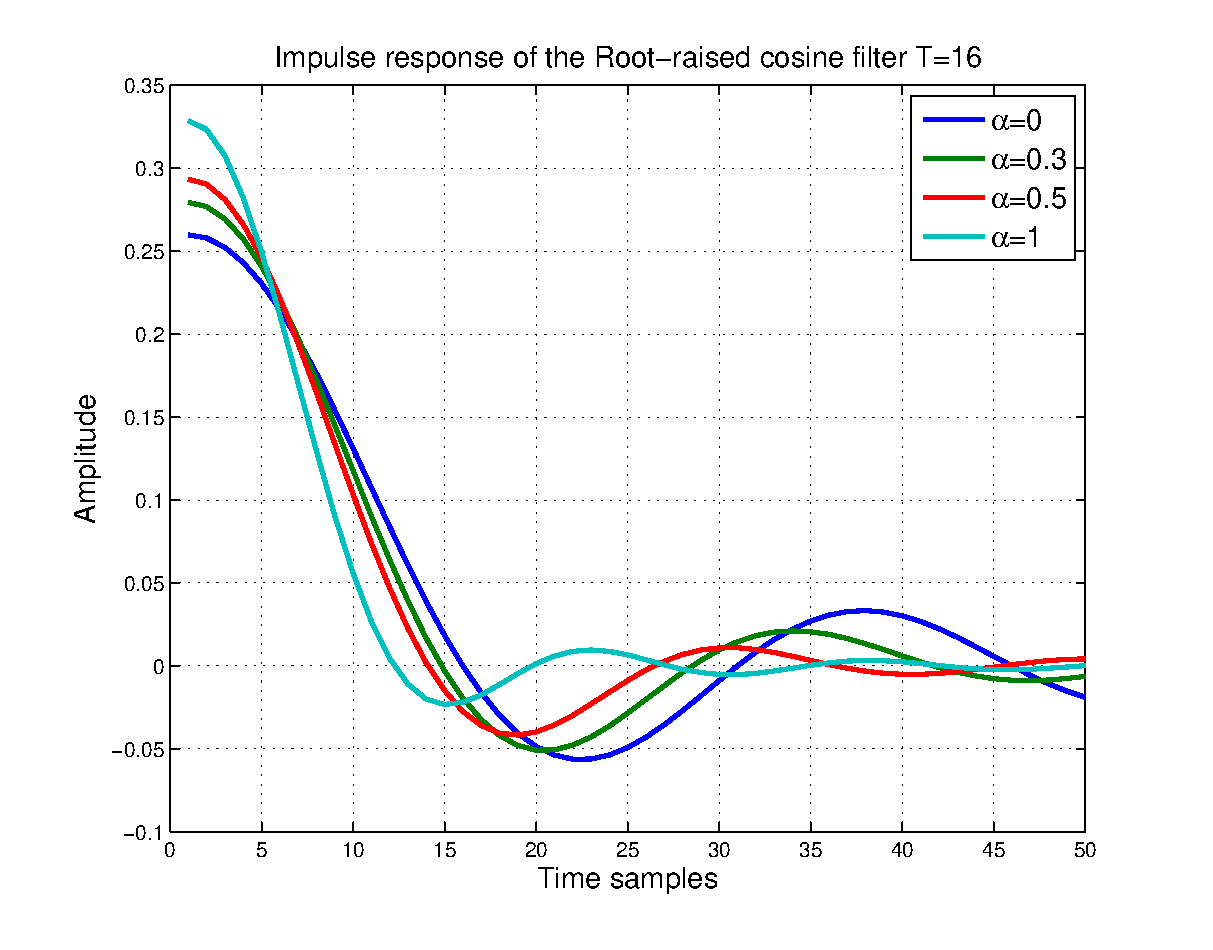
\includegraphics[width=0.9\columnwidth]{RRC_time.eps}
\caption{\textit{Impulse response of the root-raised cosine filter with different roll-off factor $\alpha$}} \label{fg_3}
\end{figure}
\begin{figure}[H]
\centering
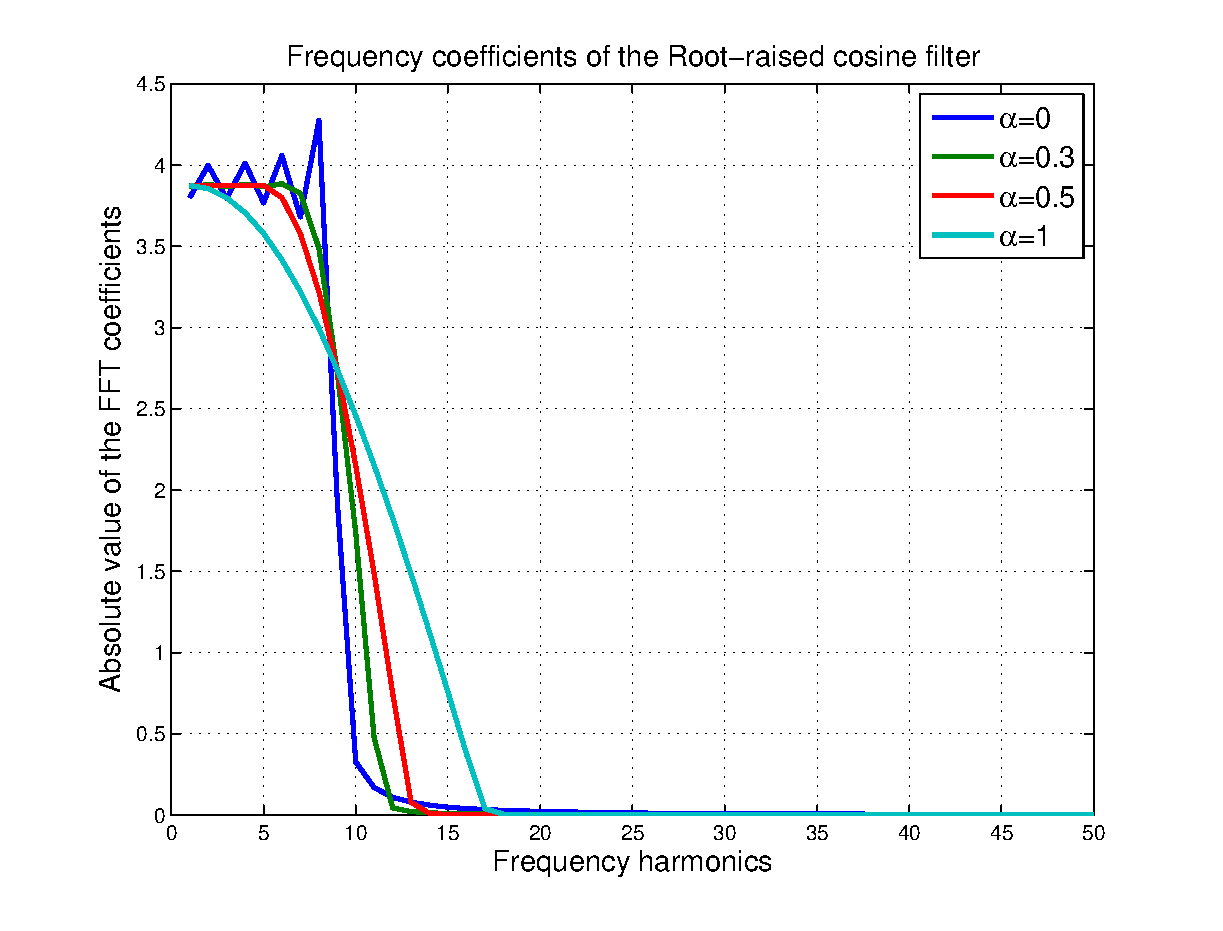
\includegraphics[width=0.9\columnwidth]{RRC_freq.eps}
\caption{\textit{Frequency envelope of the root-raised cosine filter with different roll-off factor $\alpha$}} \label{fg_4}
\end{figure}
\begin{align}
\begin{matrix}
h(t) &=& \left\{ \begin{matrix} 
\frac{1-\alpha +4\alpha/\pi}{\sqrt{T}}& if& t=0\\
\frac{\alpha}{\sqrt{2T}}[(1+\frac{2}{\pi})sin(\frac{\pi}{4\alpha})+(1-\frac{2}{\pi})cos(\frac{\pi}{4\alpha})] & if &t= \pm T/4\alpha\\
\frac{1}{\frac{t\pi}{\sqrt{T}}(1-\frac{4*\alpha t}{T})^2}(sin(\frac{\pi t (1-\alpha)}{T})+\frac{4\alpha t}{T} cos(\frac{\pi t (1+ \alpha)}{T}) ) &otherwise \\
\end{matrix} \right.
\end{matrix}
\label{g_2}
\end{align}

The comparison between the  $sinc$, raised cosine and root-raised cosine filter is shown in the fig. \ref{fg_5}. As we can see the overlap in the frequency domain spread energy from the symbol over the higher frequency range than for the $sinc$ filter \ref{fg_6}.
\begin{figure}[H]
\centering
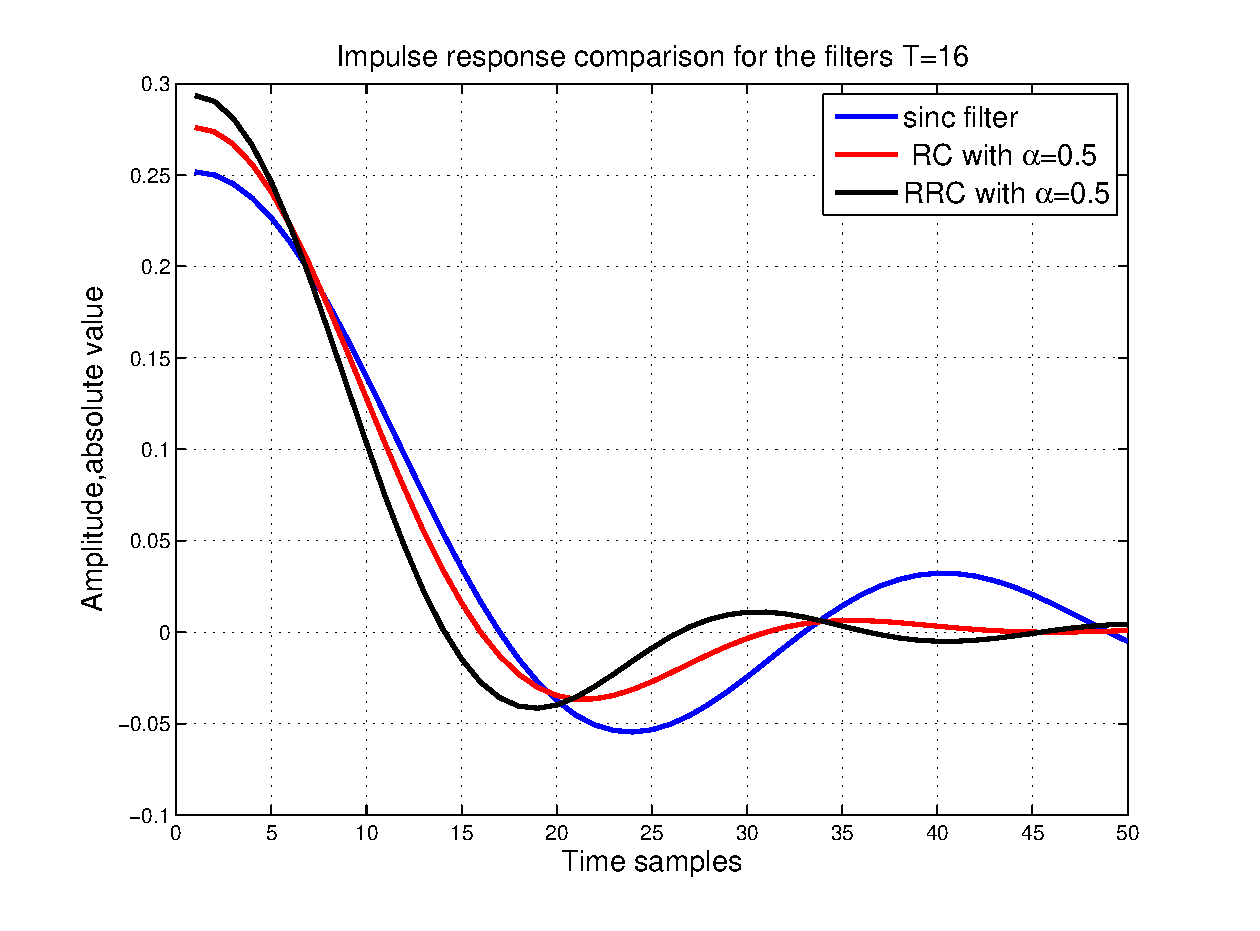
\includegraphics[width=0.9\columnwidth]{TIME_comp.eps}
\caption{\textit{Comparison between raised cosine root-raised cosine and sinc filter in the time domain}} \label{fg_5}
\end{figure}
\begin{figure}[H]
\centering
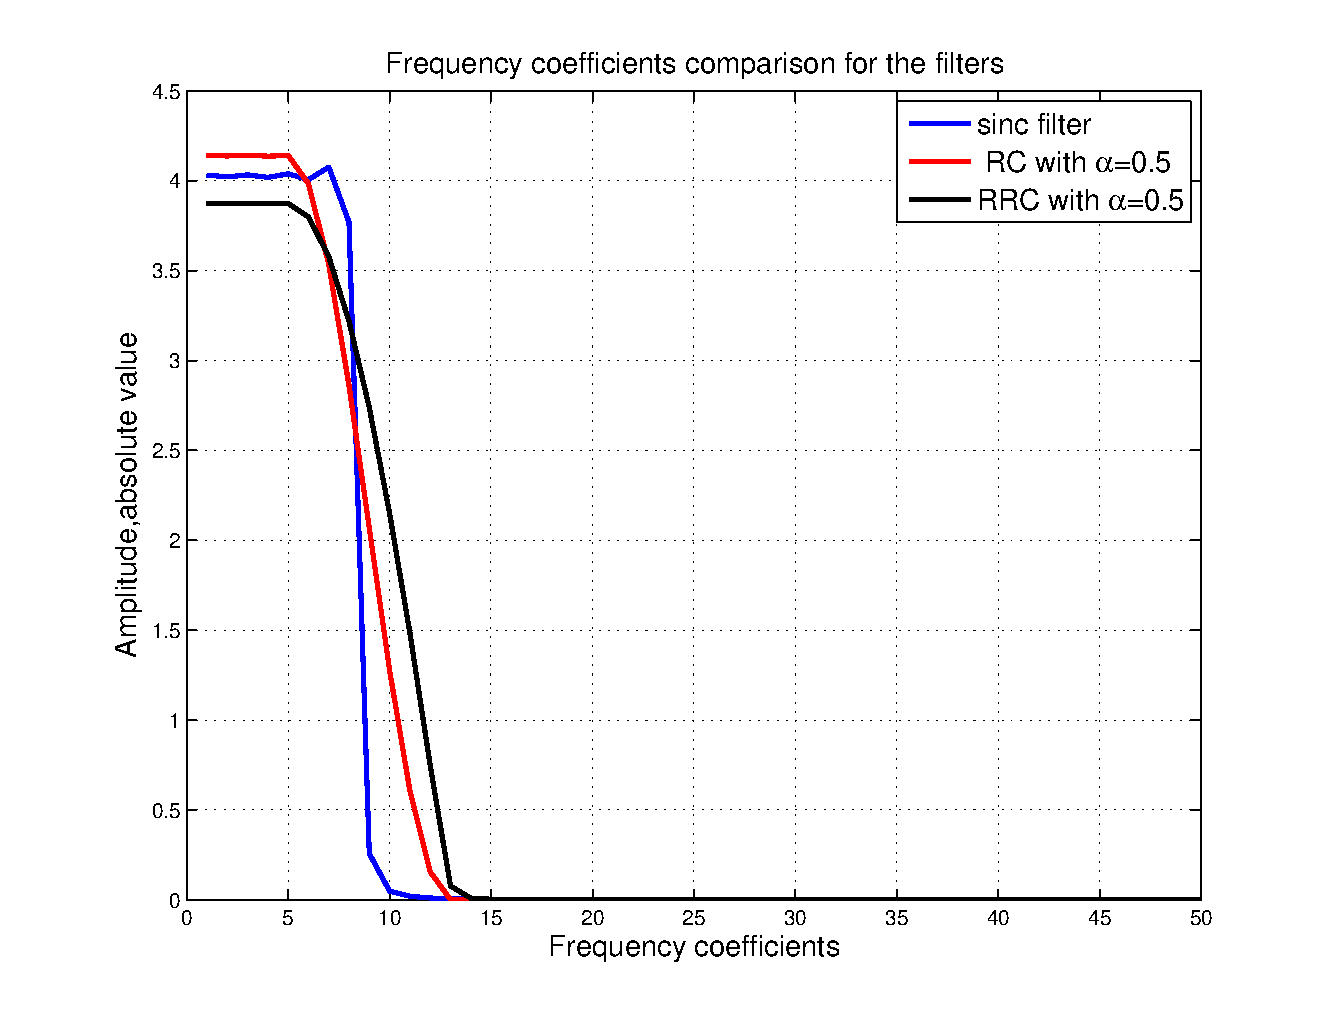
\includegraphics[width=0.9\columnwidth]{FREQ_comp.eps}
\caption{\textit{Comparison between raised cosine root-raised cosine and sinc filter in the frequency domain }} \label{fg_6}
\end{figure}

%\section{Iterative soft threshold optimization algorithm}\label{sec:ISTA}
%One of the most frequently solved tasks is deconvolution problem. The problem in the original form is written in the following equation \eqref{ista_1}. There are many ways to solve this problem in the second norm sense, with regularization and others additional algorithms. The problem in the deconvolution problem is very high conditional number of the matrix $\mathbf{H}$ which increase significantly the noise influence in the solution\cite{Book28}.
%\begin{align}
%R(x)=\mid\mid\mathbf{y}-\mathbf{Ax}\mid\mid^2_2 
%\label{ista_1}
%\end{align}
%\begin{align}
%R(x)=(\mathbf{y}-\mathbf{Ax})^H(\mathbf{y}-\mathbf{Ax})
%\label{ista_2}
%\end{align}
% In the most usual case algorithm should find the matrix inverse or pseudo inverse to solve the problem. In the paper \cite{Book27} was proposed another solution. We can find the iterative solution which will certainly decrease residual between the original and the reconstructed data from iteration to iteration. The main approach used in the algorithm called majoriziation-minimization \cite{Book27}. The approach replace the difficult problem by a number of easier minimization problems. Each minimization problem provide the answer for the solution, each next answer will be the closer to the right solution. We add additional non negative value to the original objective function to make problem easier. There are certain requirements for the majorization function $J_{add}(\mathbf{x})$. The $J_{add}(\mathbf{x})$ function must satisfy equation $J_{add}(\mathbf{x})\geq R(\mathbf{x})$ for all $x$ and moreover function must be equal in the certain point $J_{add}(\mathbf{x_k})= R(\mathbf{x_k})$. The function $J_{add}(\mathbf{x})$ can be different in the each certain point $\mathbf{x_k}$ and must be minimized easily. The explained below approach called "The Lanweber iteration". In the original form it was written for the real values function but we extend the algorithm for the complex valued functions. Assume the $J_{add}$ defined in the \eqref{ista_6}. In that case $ R_1(\mathbf{x})$ will be written as \eqref{ista_7} where $\alpha$ is some constant with is equal or higher to the maximal eigenvalue of the $\mathbf{A}^H\mathbf{A}$.  Rewrite the equation in the simpler form by opening the brackets \eqref{ista_10}. 
% \begin{align}
% R(\mathbf{x_{k+1}})<R(\mathbf{x_k})
% \label{ista_3}
% \end{align}
%\begin{align}
% R_1(\mathbf{x})=R(\mathbf{x})+J_{add}(\mathbf{x}) \label{ista_4}
%\end{align}
%\begin{align}
% R_1(\mathbf{x})=\mid\mid\mathbf{y}-\mathbf{Ax}\mid\mid^2_2+J_{add}(\mathbf{x})\label{ista_5}
%\end{align}
%\begin{align}
%J_{add}(\mathbf{x})=(\mathbf{x-x_k})^T(\alpha \mathbf{I}-\mathbf{A}^T\mathbf{A})(\mathbf{x-x_k})\label{ista_6}
%\end{align}
%\begin{align}
% R_1(\mathbf{x})=\mid\mid\mathbf{y}-\mathbf{Ax}\mid\mid^2_2+(\mathbf{x-x_k})^H(\alpha \mathbf{I}-\mathbf{A}^H\mathbf{A})(\mathbf{x-x_k}) \label{ista_7}
%\end{align}
%\begin{align}
% R_1(\mathbf{x})=(\mathbf{y}-\mathbf{Ax})^H(\mathbf{y}-\mathbf{Ax})+(\mathbf{x}-\mathbf{x}_k)^H(\alpha \mathbf{I}-\mathbf{A}^H\mathbf{A})(\mathbf{x}-\mathbf{x}_k) \label{ista_8}
%\end{align}
%\begin{align}
%\alpha \geq max(eig(\mathbf{A}^H\mathbf{A})) \label{ista_9}
%\end{align}
%\begin{align}
%R_1(\mathbf{x})=\mathbf{y}^H\mathbf{y} -\mathbf{y}^H\mathbf{A}\mathbf{x} -\mathbf{x}^H \mathbf{A}^H\mathbf{y} +\mathbf{x}^H\mathbf{A}^H\mathbf{A}\mathbf{x} \label{ista_10}
%\end{align}
%\begin{align*}
% +\mathbf{x}_k^H(\alpha \mathbf{I}-\mathbf{A}^H\mathbf{A})\mathbf{x}_k +\mathbf{x}^H(\alpha \mathbf{I}-\mathbf{A}^H\mathbf{A})\mathbf{x} 
%\end{align*}
%\begin{align*}
%-\mathbf{x}_k^H(\alpha \mathbf{I}-\mathbf{A}^H\mathbf{A})\mathbf{x} -\mathbf{x}^H(\alpha \mathbf{I}-\mathbf{A}^H\mathbf{A})\mathbf{x}_k 
%\end{align*}
%Equate the partial derivative to the zero \eqref{ista_12}. Because of the non holomorphic objective function, we take derivative with respect to the $\mathbf{x}^*$. During the transformations we can define \eqref{ista_14} the $\mathbf{x}$ from the known variables and explicitly write the equation to change $\mathbf{x}_k$ from iteration to iteration \eqref{ista_15}.
%\begin{align}
%\frac{\delta R_1(x)}{\delta x^*}=-\mathbf{A}^H\mathbf{y} +\mathbf{A}^H\mathbf{A}\mathbf{x} +(\alpha \mathbf{I}-\mathbf{A}^H\mathbf{A})\mathbf{x} -(\alpha \mathbf{I}-\mathbf{A}^H\mathbf{A})\mathbf{x}_k \label{ista_11}
%\end{align}
%\begin{align}
%\frac{\delta R_1(x)}{\delta x^*}=-\mathbf{A}^H\mathbf{y} +\alpha\mathbf{x} -\alpha\mathbf{x}_k+\mathbf{A}^H\mathbf{A}\mathbf{x}_k=0 \label{ista_12}
%\end{align}
%\begin{align}
%\mathbf{A}^H(\mathbf{y} -\mathbf{A}\mathbf{x}_k) +\alpha\mathbf{x}_k =\alpha\mathbf{x} \label{ista_13}
%\end{align}
%\begin{align}
%\mathbf{x}=\frac{\mathbf{A}^H}{\alpha}(\mathbf{y} -\mathbf{A}\mathbf{x}_k) +\mathbf{x}_k \label{ista_14}
%\end{align}
%\begin{align}
%\mathbf{x}_{k+1}=\frac{\mathbf{A}^H}{\alpha}(\mathbf{y} -\mathbf{A}\mathbf{x}_k) +\mathbf{x}_k \label{ista_15}
%\end{align}
%The defined equation \eqref{ista_15} allow to us write the optimization algorithm with high convergence speed and low computational complexity. Also there is one modification of the ISTA called FISTA which allow increase convergence speed for the one order.
%The FISTA algorithm comparing to the ISTA is similar to the CG algorithm in comparison with the SD\cite{Book28}. The FISTA works in the few steps:
%\begin{itemize}
%\item Set the start point $\mathbf{x}_0$ and set additional variable $t_0=1,t_1=1$
%\item Calculate $t_1$ via \eqref{ista_16}
%\item Take $y_1=x_0$
%\item Solve equation \eqref{ista_17} for the first iteration.
%\item Put $t_0=t_1$
%\item $y_{k+1}=x_k+(\frac{t_0-1}{t_1})(x_k-x_{k-1})$
%\item Check is the step size less than tolerance if no, go to step 2
%\end{itemize}
%\begin{align}
%t_1=\frac{1+\sqrt{1+4t_1}}{2} \label{ista_16}
%\end{align}
%\begin{align}
%\mathbf{x}_{k+1}=\frac{\mathbf{A}^H}{\alpha}(\mathbf{Y} -\mathbf{A}\mathbf{y}_k) +\mathbf{y}_k \label{ista_17}
%\end{align}
%The explained FISTA algorithm is used in the presented work in the system to solve ill-conditioned tasks for the ALS algorithm.